\section{常见统计分布}
\(\x\)分布、\(t\)分布和\(F\)分布在数理统计中与正态分布一起构成四个最基本、最重要的分布.
下面逐一介绍前三个分布.

\subsection{\texorpdfstring{\(\x\)}{卡方}分布}
\begin{definition}\label{definition:数理统计的基础知识.卡方分布的定义}
\(\AutoTuple{X}{n}\)独立同服从标准正态分布\(N(0,1)\),
称随机变量\begin{equation}
	\x = \sum_{i=1}^n{X_i^2}
\end{equation}
所服从的分布为
“自由度为\(n\)的 \DefineConcept{\(\x\)分布}”
\footnote{念作“卡方分布”.},
记为\(\x \sim \x(n)\).
\end{definition}

\begin{figure}[htb]
	\centering
	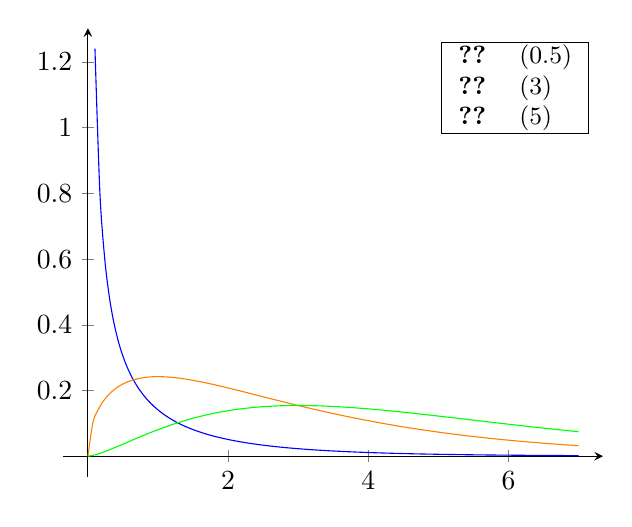
\begin{tikzpicture}
		\begin{axis}[
			name=ChiSquareDistribution,
			axis y line=middle,
			axis x line=middle,
			enlarge x limits=0.05,
			enlarge y limits=0.05,
			xscale=1,
		]
			\def\plotCSDPDF#1#2#3{\addplot[color=#3,samples=100,smooth,domain=.1:7]{%首次定义
				x^(#1-1)*exp(-x/2)/(2^(#1)*#2)
			}}%
			\plotCSDPDF{.25}{3.62561}{blue};\label{pgfplots:卡方分布.Chi^2(.5)}
			\def\plotCSDPDF#1#2#3{\addplot[color=#3,samples=100,smooth,domain=0:7]{%重新定义
				x^(#1-1)*exp(-x/2)/(2^(#1)*#2)
			}}%
			\plotCSDPDF{1.5}{0.886227}{orange};\label{pgfplots:卡方分布.Chi^2(3)}
			\plotCSDPDF{2.5}{1.32934}{green};\label{pgfplots:卡方分布.Chi^2(5)}
		\end{axis}
		\node[draw,fill=white,inner sep=0pt,below left=0.5em]
		at(ChiSquareDistribution.north east){\small\begin{tabular}{cl}
			\ref{pgfplots:卡方分布.Chi^2(.5)} & \(\x(0.5)\) \\
			\ref{pgfplots:卡方分布.Chi^2(3)} & \(\x(3)\) \\
			\ref{pgfplots:卡方分布.Chi^2(5)} & \(\x(5)\) \\
		\end{tabular}};
	\end{tikzpicture}
	\caption{\(\x\)分布的密度函数}
\end{figure}

\begin{theorem}\label{theorem:数理统计的基础知识.卡方分布的密度函数}
\(\x(n)\)分布等价于\(\Gamma\left(\frac{n}{2},\frac{1}{2}\right)\)分布,
其密度函数为\begin{equation}
	f(x,n) = \left\{ \begin{array}{cl}
		\frac{1}{2^{n/2} \Gamma(n/2)} x^{\frac{n}{2}-1} e^{-\frac{x}{2}}, & x > 0, \\
		0, & x \leq 0.
	\end{array} \right.
\end{equation}
\begin{proof}
首先求\(Z=X_1^2\)的分布.
由于\(Z\)非负,故当\(z \leq 0\)时,
\(P(Z \leq z) = 0\);
当\(z > 0\)时,\(Z\)的分布函数为\[
	F_Z(z) = P(Z \leq z)
	= P(X_1^2 \leq z)
	= P(-\sqrt{z} \leq X_1 \leq \sqrt{z})
	= \Phi(\sqrt{z}) - \Phi(-\sqrt{z}),
\]
其中\(\Phi\)是标准正态分布的分布函数.
于是\(Z\)的密度函数为\[
	f_Z(z)
	= F_Z'(z)
	= \frac12 z^{-\frac12} \left[
		\phi(\sqrt{z}) + \phi(-\sqrt{z})
	\right],
\]
其中\(\phi(x) = \frac{1}{\sqrt{2\pi}} \exp(-\frac{x^2}{2})\)为标准正态分布的密度函数.
代入即得\[
	f_Z(z) = \left\{ \begin{array}{cl}
		\frac{1}{\sqrt{2\pi}} z^{-\frac12} e^{-\frac{z}{2}}, & z>0, \\
		0, & z \leq 0.
	\end{array} \right.
\]
这正是\(\Gamma\left(\frac12,\frac12\right)\)的密度函数.

又因为\(\AutoTuple{X}{n}\)独立同分布,
所以\(\AutoTuple{X^2}{n}\)也独立同分布于\(\Gamma\left(\frac12,\frac12\right)\).

再由~\hyperref[theorem:多维随机变量及其分布.伽马分布的可加性1]{\(\Gamma\)分布的可加性}可知
\(\x = X_1^2+X_2^2+\dotsb+X_n^2\)服从\(\Gamma\left(\frac{n}{2},\frac12\right)\).
\end{proof}
\end{theorem}

因为\(\x(n)=\Gamma\left(\frac{n}{2},\frac12\right)\),
所以由\cref{theorem:期望.伽马分布的期望,theorem:方差.伽马分布的方差}
可以得到卡方分布的数学期望和方差.
\begin{corollary}\label{theorem:数理统计的基础知识.卡方分布的数字特征}
%@see: 《概率论与数理统计》(茆诗松、周纪芗、张日权) P101 例2.4.8
设\(\x \sim \x(n)\),则
\begin{gather}
	E(\x) = n, \\
	D(\x) = 2n.
\end{gather}
\end{corollary}

\begin{theorem}[可加性]\label{theorem:数理统计的基础知识.卡方分布的可加性1}
设\(\x_1 \sim \x(n_1)\),\(\x_2 \sim \x(n_2)\),
且\(\x_1\)与\(\x_2\)相互独立,则\begin{equation}
	\x_1 + \x_2 \sim \x(n_1+n_2).
\end{equation}
\begin{proof}
因为\[
	\x(n_1) = \Gamma\left(\frac{n_1}{2},\frac12\right), \qquad
	\x(n_2) = \Gamma\left(\frac{n_2}{2},\frac12\right),
\]
所以,根据\hyperref[theorem:多维随机变量及其分布.伽马分布的可加性1]{伽马分布的可加性}可知\[
	\x_1 + \x_2 \sim \Gamma\left(\frac{n_1+n_2}{2},\frac12\right)
	= \x(n_1+n_2).
	\qedhere
\]
\end{proof}
\end{theorem}

\begin{corollary}\label{theorem:数理统计的基础知识.卡方分布的可加性2}
设随机变量序列\(\x_k \sim \x(n_k)\ (k=1,2,\dotsc,n)\),
且\(\x_1,\x_2,\dotsc,\x_n\)相互独立,则\begin{equation}
	\sum_{k=1}^n \x_k \sim \x\left(\sum_{k=1}^n{n_k}\right).
\end{equation}
\end{corollary}

\subsection{\texorpdfstring{\(t\)}{t}分布}
\begin{definition}
设随机变量\(X \sim N(0,1)\),\(Y \sim \x(n)\),
且\(X\)与\(Y\)相互独立,称随机变量\begin{equation}
	t = \frac{X}{\sqrt{Y/n}}
\end{equation}
所服从的分布为
“自由度为\(n\)的~\DefineConcept{\(t\)分布}”
\footnote{又作“学生氏分布”.},
记为\(t \sim t(n)\).
\end{definition}

\begin{theorem}\label{theorem:数理统计的基础知识.学生氏分布的密度函数}
\(t\)分布的密度函数为\begin{equation}
	t(x,n) = \frac{
		\Gamma\left(\frac{n+1}{2}\right)
	}{
		\sqrt{n\pi} \cdot \Gamma\left(\frac{n}{2}\right)
	}
	\left(1+\frac{x^2}{n}\right)^{-\frac{n+1}{2}},
	\quad x \in \mathbb{R}.
\end{equation}
\end{theorem}

由于\(t\)分布的密度函数\(t(x,n)\)是偶函数,容易验证:
当\(n=1\)时\(t\)分布的数学期望\(E(t)\)不存在,
而当\(n \geq 2\)时数学期望\(E(t)=0\).

当自由度\(n\to\infty\)时,有\[
	\lim_{n\to\infty} t(x,n) = \frac{1}{\sqrt{2\pi}} e^{-\frac{x^2}{2}},
	\quad x \in \mathbb{R}.
\]
当\(n\)充分大时(通常需要\(n \geq 45\)),
\(t\)分布就近似于标准正态分布\(N(0,1)\).

\subsection{\texorpdfstring{\(F\)}{F}分布}
\begin{definition}
设随机变量\(X \sim \x(n)\),\(Y \sim \x(m)\),且\(X\)与\(Y\)独立,
称随机变量\begin{equation}
	F=\frac{X/n}{Y/m}
\end{equation}
所服从的分布为
“自由度为\((n,m)\)的 \DefineConcept{\(F\)分布}”,
记为\(F \sim F(n,m)\),
其中\(n\)称为\DefineConcept{第一自由度}(或\DefineConcept{分子自由度}),
\(m\)称为\DefineConcept{第二自由度}(或\DefineConcept{分母自由度}).
\end{definition}

\begin{proposition}
\(F \sim F(n,m) \implies \frac{1}{F} \sim F(m,n)\).
\end{proposition}

\begin{theorem}
\(F\)分布的密度函数为\begin{equation}
	f(x,n,m) = \left\{ \begin{array}{cl}
		A(n,m) \cdot x^{\frac{n}{2}-1}
		\left(1+\frac{n}{m}x\right)^{-\frac{n+m}{2}},
		& x > 0, \\
		0, & x \leq 0,
	\end{array} \right.
\end{equation}
其中\[
	A(n,m)=\frac{
		\Gamma\left(\frac{n+m}{2}\right)
	}{
		\Gamma\left(\frac{n}{2}\right) \Gamma\left(\frac{m}{2}\right)
	}
	\left(\frac{n}{m}\right)^{\frac{n}{2}}.
\]
\end{theorem}

\begin{example}
设\(X \sim t(n)\),\(Y=\frac{1}{X^2}\).
求\(Y\)的分布.
\begin{solution}
由题意有\(X = \frac{U}{\sqrt{V/n}}\),
其中\(U \sim N(0,1)\),\(V \sim \x(n)\),且\(U\)与\(V\)相互独立.
因此\[
	Y = \frac{V/n}{U^2}.
\]
由于\(U^2 \sim \x(1)\),
所以\(Y \sim F(n,1)\).
\end{solution}
\end{example}
